\documentclass[aspectratio=169,11pt]{beamer}
\def\courseweek{8}
% Shared style for the Introduction to Information Geometry lecture slides.
% Compile the lecture .tex files from this directory.
\providecommand{\courseweek}{1}
\usepackage[T1]{fontenc}
\usepackage[utf8]{inputenc}
\usepackage[sc]{mathpazo}
\renewcommand{\sfdefault}{lmss}
\renewcommand{\ttdefault}{lmtt}
\usepackage{amsmath,amssymb,mathtools}
\usepackage{tikz}
\usetikzlibrary{arrows.meta,calc,positioning}
\usepackage{pgfplots}
\pgfplotsset{compat=1.18}
\usepackage{booktabs}

\definecolor{courseink}{HTML}{173749}
\definecolor{coursemuted}{HTML}{526674}
\definecolor{courseteal}{HTML}{0E7287}
\definecolor{coursecopper}{HTML}{B66B43}
\definecolor{courseline}{HTML}{D4E0E3}
\definecolor{coursepale}{HTML}{EFF5F5}

\setbeamercolor{normal text}{fg=courseink,bg=white}
\setbeamercolor{structure}{fg=courseteal}
\setbeamercolor{frametitle}{fg=courseink,bg=white}
\setbeamercolor{title}{fg=courseink}
\setbeamercolor{subtitle}{fg=coursemuted}
\setbeamercolor{block title}{fg=courseink,bg=white}
\setbeamercolor{block body}{fg=courseink,bg=white}
\setbeamercolor{alerted text}{fg=coursecopper}
\setbeamerfont{title}{family=\rmfamily,series=\bfseries,size=\fontsize{32}{37}}
\setbeamerfont{frametitle}{family=\rmfamily,series=\bfseries,size=\fontsize{26}{31}}
\setbeamerfont{normal text}{size=\fontsize{18}{22}}
\setbeamerfont{subtitle}{size=\fontsize{17}{21}}
\setbeamersize{text margin left=0.78cm,text margin right=0.78cm}
\setbeamertemplate{navigation symbols}{}
\setbeamertemplate{itemize items}[circle]
\setbeamertemplate{enumerate items}[default]
\setbeamertemplate{blocks}[default]
\setlength{\parskip}{0.22em}
\setbeamertemplate{footline}{%
  \leavevmode\hbox to \paperwidth{\hspace{.78cm}%
  {\color{coursemuted}\fontsize{8.5}{10}\selectfont Introduction to Information Geometry \hspace{.32cm} / \hspace{.32cm} Week \courseweek}%
  \hfill{\color{coursemuted}\fontsize{8.5}{10}\selectfont \insertframenumber\hspace{.17cm}/\hspace{.17cm}\inserttotalframenumber}\hspace{.78cm}}%
  \vskip.17cm
}
\setbeamertemplate{frametitle}{%
  \vspace{.13cm}
  \insertframetitle\par
  \vspace{.08cm}
}
\setbeamertemplate{title page}{%
  \vspace*{1.00cm}
  {\color{courseteal}\fontsize{10}{13}\selectfont\bfseries
  INTRODUCTION TO INFORMATION GEOMETRY\par}
  \vspace{.40cm}
  {\usebeamerfont{title}\usebeamercolor[fg]{title}\inserttitle\par}
  \vspace{.22cm}
  {\usebeamerfont{subtitle}\usebeamercolor[fg]{subtitle}\insertsubtitle\par}
  \vfill
  {\color{coursemuted}\fontsize{13}{16}\selectfont Christopher Lee\par}
  \vspace{.34cm}
}

\pgfplotsset{
  courseplot/.style={
    width=11.05cm,
    height=5.15cm,
    axis line style={coursemuted!75},
    tick style={coursemuted!65},
    ticklabel style={font=\scriptsize,color=coursemuted},
    label style={font=\normalsize,color=courseink},
    grid=major,
    major grid style={courseline!70,line width=.4pt},
    line width=1.45pt,
    legend style={font=\small,draw=none,fill=none,at={(.98,.03)},anchor=south east},
    clip=true
  }
}

\newcommand{\highlightmath}[1]{{\color{courseteal}#1}}
\newcommand{\thinrule}{\par\vspace{.25cm}{\color{courseline}\rule{\linewidth}{.8pt}}\par}

% A one-dimensional state space.  x=0 and x=1 are placed at 0 and 9 units.
\newcommand{\stateinterval}[1]{%
 \begin{tikzpicture}[x=1cm,y=1cm]
   \draw[courseink,line width=1.25pt] (0,0)--(9,0);
   \foreach \pos/\lab in {0/0,9/1} {
     \fill[courseink] (\pos,0) circle(2.7pt);
     \node[below=9pt,text=coursemuted] at (\pos,0) {\(\lab\)};
   }
   #1
 \end{tikzpicture}%
}

% Paired pages are separate frames in the PDF, with matching titles.
% Supply the whole frame body for each version; the instructor may edit them
% independently without changing overlay logic.
\newcommand{\coursepair}[3]{%
  \begin{frame}{#1}#2\end{frame}%
  \begin{frame}{#1}#3\end{frame}%
}

% Equilateral representation of the categorical simplex, in barycentric
% coordinates with vertices A=(0,0), B=(1,0), C=(1/2,sqrt(3)/2).
\newcommand{\coursesimplex}[1]{%
 \begin{tikzpicture}[scale=4.9]
  \fill[coursepale] (0,0)--(1,0)--(.5,.8660254)--cycle;
  \draw[courseink,line width=.65pt] (0,0)--(1,0)--(.5,.8660254)--cycle;
  \node[below left,font=\small] at (0,0) {A};
  \node[below right,font=\small] at (1,0) {B};
  \node[above,font=\small] at (.5,.8660254) {C};
  #1
 \end{tikzpicture}%
}

\title{Square-Root Coordinates and the Sphere}
\subtitle{Week 8 \(\cdot\) Lecture 1}
\date{}
\begin{document}
\begin{frame}[plain]\titlepage\end{frame}

\begin{frame}{A new coordinate for each probability}
For an interior categorical law \(P=(p_i)\), define
\[
\highlightmath{s_i=2\sqrt{p_i}}.
\]
\vspace{.45cm}
Since \(\sum_i p_i=1\),
\[
\highlightmath{\sum_i s_i^2=4}.
\]
\vspace{.38cm}
The image lies in the positive orthant of a sphere of radius 2.
\end{frame}

\begin{frame}{Bernoulli laws form a quarter-circle}
For \(P=(p,1-p)\), the image is
\[
s(p)=(2\sqrt p,2\sqrt{1-p}).
\]
\vspace{-.48cm}
\begin{center}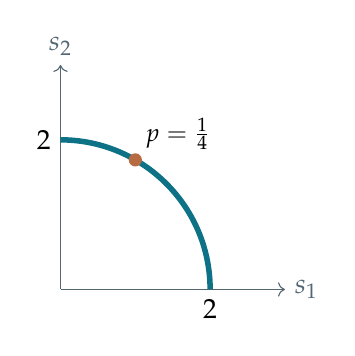
\begin{tikzpicture}[scale=.95]
\draw[->,coursemuted](0,0)--(3,0)node[right]{$s_1$};
\draw[->,coursemuted](0,0)--(0,3)node[above]{$s_2$};
\draw[courseteal,line width=2pt](2,0)arc(0:90:2);
\fill[coursecopper]({2*cos(60)},{2*sin(60)})circle(2.5pt);
\node[above right,font=\small]at(1,1.732){\(p=\tfrac14\)};
\node[below]at(2,0){2};\node[left]at(0,2){2};
\end{tikzpicture}\end{center}
\end{frame}

\coursepair{Mapping a Bernoulli law}{
Map \(P=(\frac14,\frac34)\) to square-root coordinates.
\vspace{.53cm}
\[
s=(2\sqrt{\tfrac14},2\sqrt{\tfrac34})=(\;?,\;?).
\]
\vspace{.40cm}
Check that \(\|s\|^2=4\).
}{
Map \(P=(\frac14,\frac34)\) to square-root coordinates.
\vspace{.53cm}
\[
\highlightmath{s=(1,\sqrt3)}.
\]
\vspace{.40cm}
Indeed \(\|s\|^2=1+3=4\).
}

\begin{frame}{Square roots preserve Fisher length}
Differentiate \(s_i=2\sqrt{p_i}\):
\[
ds_i=\frac{dp_i}{\sqrt{p_i}}.
\]
\vspace{.47cm}
Therefore the Euclidean squared length on the sphere is
\[
\highlightmath{\sum_i ds_i^2=\sum_i\frac{dp_i^2}{p_i}=ds_F^2}.
\]
\vspace{.41cm}
The square-root map is an isometry between the positive simplex
and the positive spherical orthant.
\end{frame}

\begin{frame}{The shortest spherical route}
For two non-antipodal points on a sphere, the shortest path is
the shorter arc of the great circle through them.
\vspace{.5cm}
On a radius-2 sphere, its length is twice the central angle:
\[
\highlightmath{d=2\alpha}.
\]
\vspace{.43cm}
Square-root images of probability laws lie in one positive orthant;
their shorter arc remains inside it.
\end{frame}

\begin{frame}{The Bhattacharyya overlap}
For two categorical laws \(P=(p_i)\) and \(R=(r_i)\), define
\[
\highlightmath{B(P,R)=\sum_i\sqrt{p_ir_i}}.
\]
\vspace{.44cm}
Their square-root vectors have dot product \(4B(P,R)\), hence
\[
\cos\alpha=B(P,R).
\]
\vspace{.38cm}
This determines Fisher distance directly from the probabilities.
\end{frame}

\begin{frame}{Fisher distance for categorical laws}
\vspace{.55cm}
\begin{center}
{\fontsize{27}{34}\selectfont
\(\displaystyle\highlightmath{d_F(P,R)=2\arccos\left(\sum_i\sqrt{p_ir_i}\right)}\)}
\end{center}
\vspace{.6cm}
The expression is symmetric and measures shortest-path length.
\end{frame}

\coursepair{An exact distance from three probabilities}{
Let \(P=(.5,.3,.2)\) and \(R=(.2,.5,.3)\).
\vspace{.39cm}
Calculate the overlap
\[
B(P,R)=\sqrt{.10}+\sqrt{.15}+\sqrt{.06}.
\]
\vspace{.34cm}
Then determine \(d_F(P,R)\).
}{
Let \(P=(.5,.3,.2)\) and \(R=(.2,.5,.3)\).
\vspace{.39cm}
The overlap is \(B\approx\highlightmath{.948475}\).
\vspace{.34cm}
\[
\highlightmath{d_F(P,R)=2\arccos B\approx.644817}.
\]
}

\begin{frame}{Boundary distributions have finite distance}
For disjoint pure outcomes, such as
\(P=(1,0)\) and \(R=(0,1)\),
\[
B(P,R)=0.
\]
\vspace{.50cm}
Thus the limiting Fisher distance is
\[
\highlightmath{d_F(P,R)=\pi}.
\]
\vspace{.43cm}
The open positive simplex can be completed by adding its boundary
at finite distance.
\end{frame}

\begin{frame}{KL divergence and Fisher distance}
KL divergence compares expected log loss and depends on direction.
\vspace{.49cm}
Fisher distance is symmetric because it is intrinsic shortest-path length.
\vspace{.49cm}
Both arise from the same local quadratic information structure.
\end{frame}
\end{document}
